\chapter{A Guideline for Developers}
\lipsum[1-2]


\section{Use \forkOn for embarrassingly parallel problems}
\sstate{Description:} Both the performance and energy consumption of a program can be improved by using \forkOn to create new threads of execution when there is little or no dependency among these threads.
\newline

\sstate{Justification:} A problem that can be decomposed into parallel tasks that do not need to communicate with each other to make progress is called \emph{embarrassingly parallel}. In this kind of problem, we can improve the program's performance by keeping each worker thread executing on a separate CPU core. As the tasks have no dependency, keeping each one on its own core reduces the costs of context-switching. The use of \forkOn does not guarantee that each Haskell thread will be kept running on the same CPU core. However, it ensures that each Haskell thread runs on the same capability during the whole execution. It disables the load balancing of these worker threads among different capabilities, which reduces the overhead incurred by the Haskell runtime system. We observed this phenomenon in the results from our study presented in \chapref{chp:study}. The benchmarks \mandelbrot, \regex and \spectral are embarrassingly parallel problems where the variants using \forkOn superseded the others.

\begin{figure*}[tp]
\caption{Energy/Time charts for \regex and \spectral using \texttt{-qa} and \texttt{-qm}}
\centering
$
\begin{array}{ccc}
 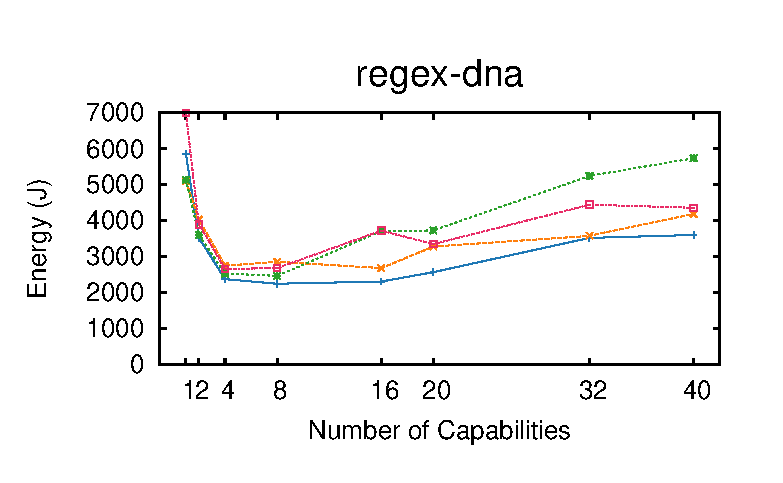
\includegraphics[width=.48\textwidth]{images/conc_bench/regex-dna-qX-energy} &
 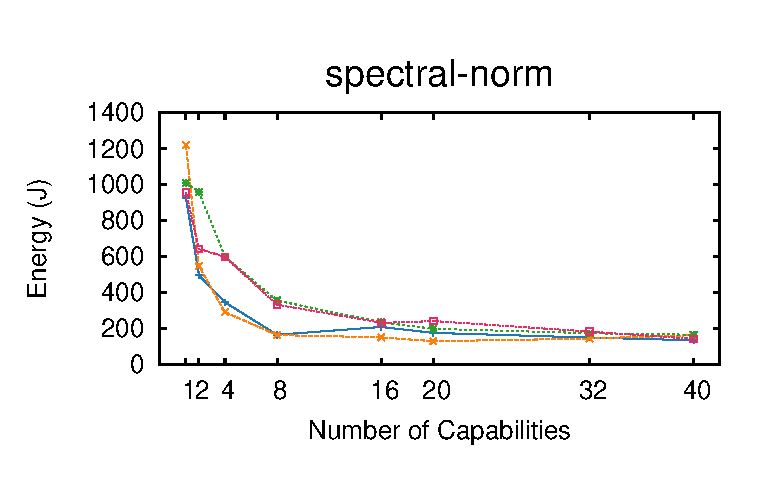
\includegraphics[width=.48\textwidth]{images/conc_bench/spectral-norm-qX-energy} \\

 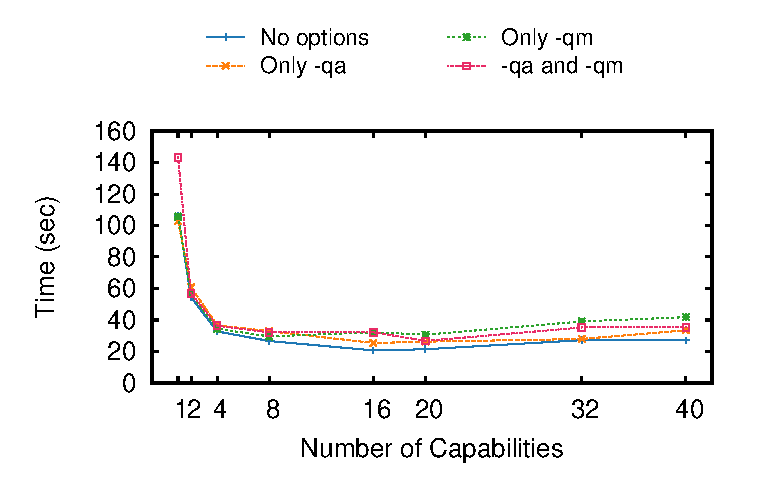
\includegraphics[width=.48\textwidth]{images/conc_bench/regex-dna-qX-time} &
 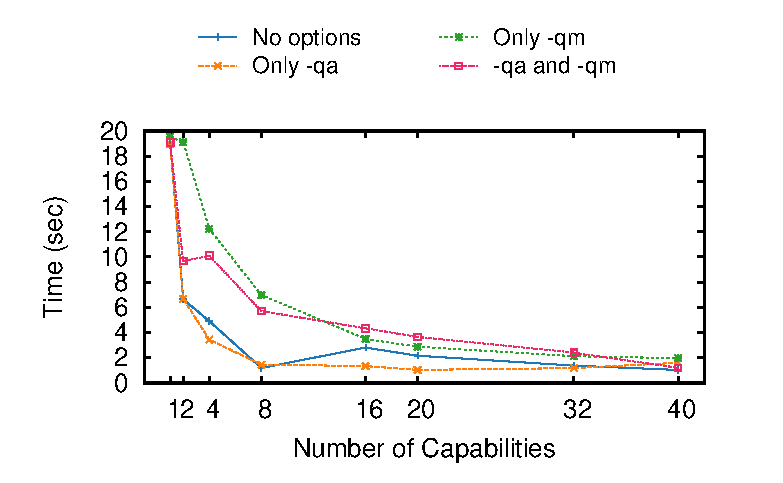
\includegraphics[width=.48\textwidth]{images/conc_bench/spectral-norm-qX-time} \\
\end{array}
$
\footnotesize{Source: Made by the author}
\label{fig:rts-flags}
\end{figure*}

Additionally, there are two \ac{rts} options that, in conjunction with \forkOn, can affect the performance of some embarrassingly parallel algorithms. The first one is the \texttt{-qa} option. It tries to pin OS threads to CPU cores using native OS facilities\footnote{In Linux, GHC uses the \texttt{sched\_setaffinity()} syscall}. Using this option, the OS threads associated with a capability \emph{i} are bound the CPU core \emph{i}. The other one is the \texttt{-qm} option. It disables automatic migration of threads between CPUs. The former seems to fit perfectly in this context since it increases the probability of a Haskell thread being kept running on the same CPU core during the execution of the program. The latter, however, it is not clear how different it is from simply creating all threads with \forkOn as we are proposing here. To get a picture of their influence, we executed our embarrassingly parallel benchmarks with these options. In \figref{fig:rts-flags} we show results for the \forkOn-\MVar variant of both \regex and \spectral. Here, we executed the benchmarks without either of the options, only with \texttt{-qa}, only with \texttt{-qm} and with both options. As we can see, the \ac{rts} options affect the performance of both benchmarks. However, the behavior is not predictable. In \spectral, using only \texttt{-qa} improves both performance and energy consumption regardless of the number of capabilities. In \regex, however, using any combination of the \ac{rts} options have a negative impact on performance. It also increases considerably the energy consumption for more than eigth capabilities. We recommend developers to experiment with these options to assess how they affect the performance of a given program.


% XXX: may change this tip to suggest the number of capabilities to be used?
\section{Avoid setting more capabilities than available CPUs}
\sstate{Description:} [[ TODO ]]
\newline

\sstate{Justification:} [[ TODO ]]


\section{Avoid using \forkOS to spawn new threads}
\sstate{Description:} [[ TODO ]]
\newline

\sstate{Justification:} [[ TODO ]]
